\documentclass{udpreport}
\documentclass{article}
\usepackage[export]{adjustbox}
\title{Ruteo estático y dinámico. }
\author{Integrantes: Thomas Muñoz, Ignacio Yanjari, Dagoberto Navarrete, Ignacio López.}
\date{17 de Julio de 2016}
\usepackage{graphicx}
\usepackage{float}
\graphicspath{ {images/} }
\udpschool{Escuela de Informática y Telecomunicaciones}

\begin{document}
\maketitle
\tableofcontents
\listoffigures
\chapter{Introducción}
  En este laboratorio tenemos como objetivo aprender a hacer funcionar de forma correcta una red para que las subredes de esta se
  pueden comunicar entre ellas, entender en que consiste el ruteo estático y el ruteo dinámico, cuáles son sus diferencias y las
  ventajas y desventajas de cada uno, también aprenderemos como configurar una red con cada tipo de ruteo y dentro del ruteo dinámico
  veremos lo que son los protocolos de enrutamiento, enfocándonos en RIP (Routing Information Protocol).
\chapter{Actividades}
	\section{Topología base}
	Lo primero que se procedió a hacer es abrir el Cisco Packet Tracer, posteriormente se continua a sacar ocho ordenadores,
	cuatro switch y cuatro routers. Una vez con los dispositivos en la interfaz se continua a posicionarlos en el espacio de
	manera que quedaran como la topología mostrada, luego se conectaron los ordenadores a los switch y los switch a los
	routers, hecho esto se procede a instalar el modulo serial en los routers, por lo que eran apagados y luego se les insertaba
	el modulo. Hecho lo anterior se procede a conectar los router entre si esto se logra a través de un cable serial, una vez
	terminado esto se continua a seguir con las actividades posteriores.\\
	\begin{figure}[H]
	\centering
	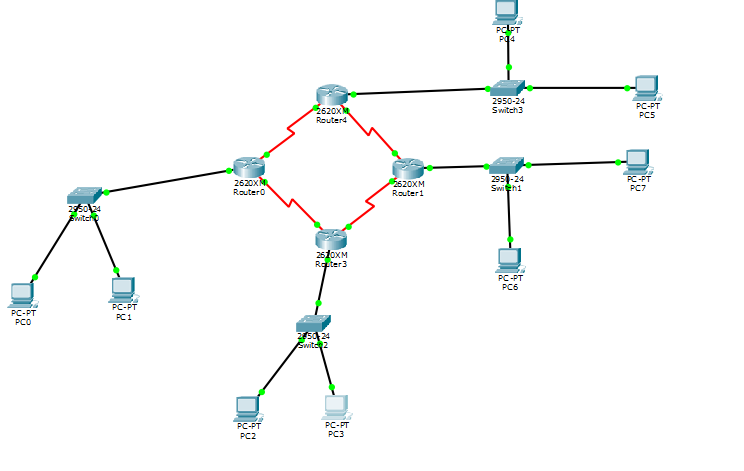
\includegraphics[width=\textwidth]{Topologia_base.PNG}
	\caption{Construccion de la Topología Base}
	\end{figure}\\	
	\section{Configuracion Equipos}
	Se configuran los equipos de manera que cada PC pertenezca a una red distinta, esto se hace en las configuraciones de cada PC
	donde se le asignan IPs manualmente, y luego se configura el router asignándole una IP perteneciente a la red común con los 
	PC.\\
	\begin{figure}[H]
	\centering
	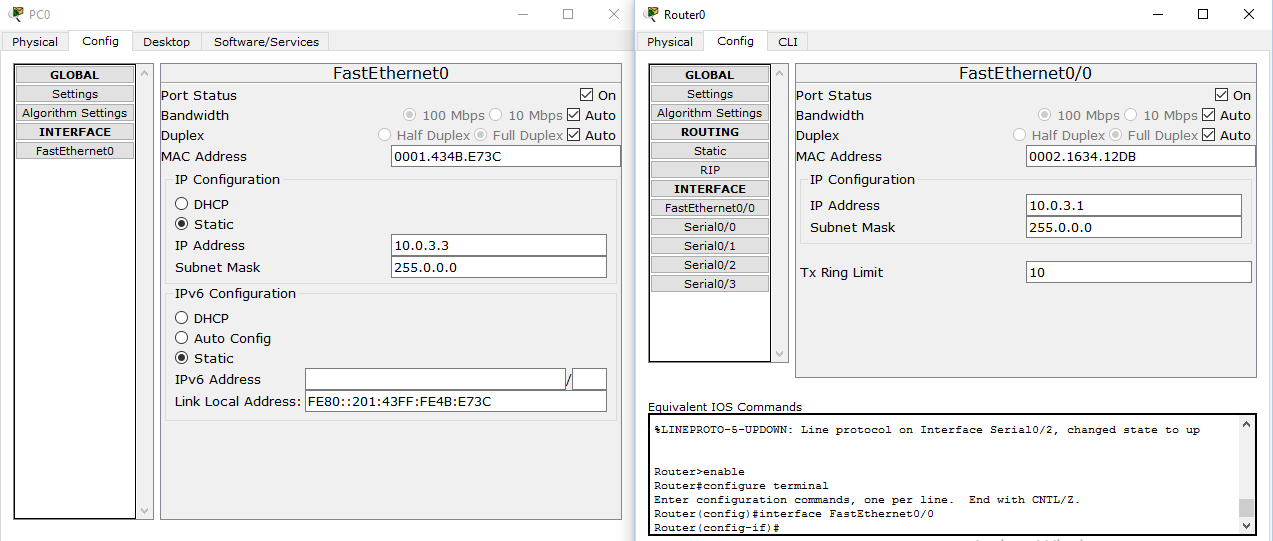
\includegraphics[width=\textwidth]{Configuracion_equipos.PNG}
	\caption{Configuracion de los equipos}
	\end{figure}\\
	\section{Configuracion ruteo estático}
	Se ingresa a la terminal del router, luego indicándoles la IP de destino, porque puerto sale, y la IP por donde da el salto
	para llegar a destino, esto se debe hacer con cada interfaz del router, de manera que dirija cada paquete que reciba a una
	interfaz y lo pueda enviar. Lo anterior descrito se debe hacer con cada router perteneciente a la topología, para que así las
	redes queden todas conectadas entre sí.\\
	\begin{figure}[H]
	\centering
	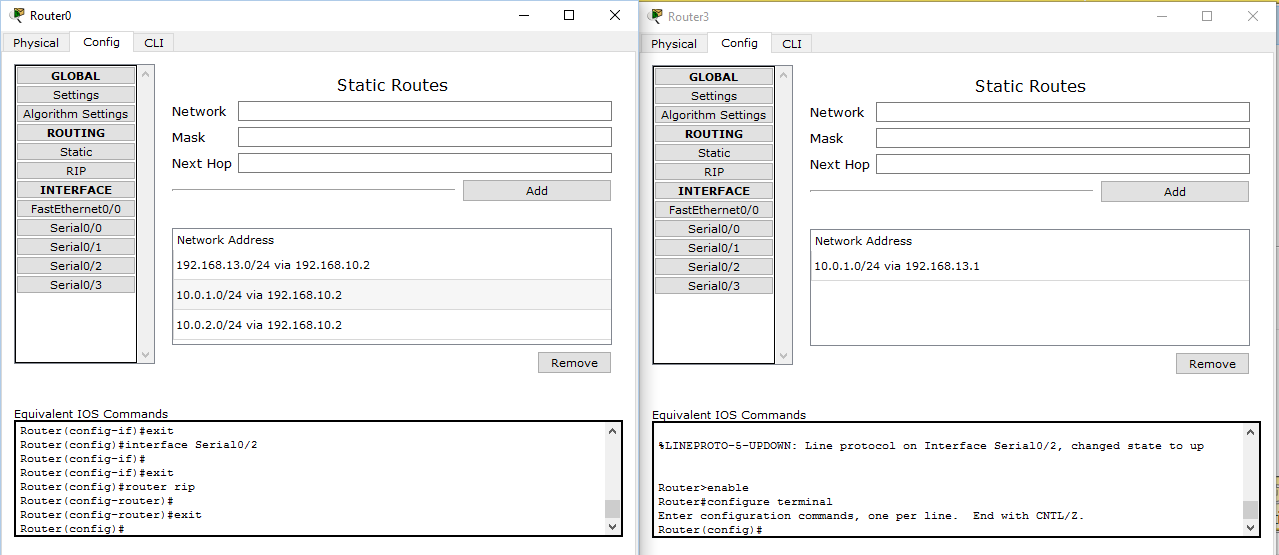
\includegraphics[width=\textwidth]{Ruteo_estatico.PNG}
	\caption{Configuracion de ruteo estatico en los router R0 y R3}
	\end{figure}\\
	\section{Configuracion ruteo dinámico}
	Se ingresa a la terminal del router y se activa RIP V1 de esta manera se configura automáticamente y solo tenemos que
	indicarle al router cuál es la red que va a utilizar. Esto se logra al ingresar los comandos que estaban especificados en la
	guía.\\
	\begin{figure}[H]
	\centering
	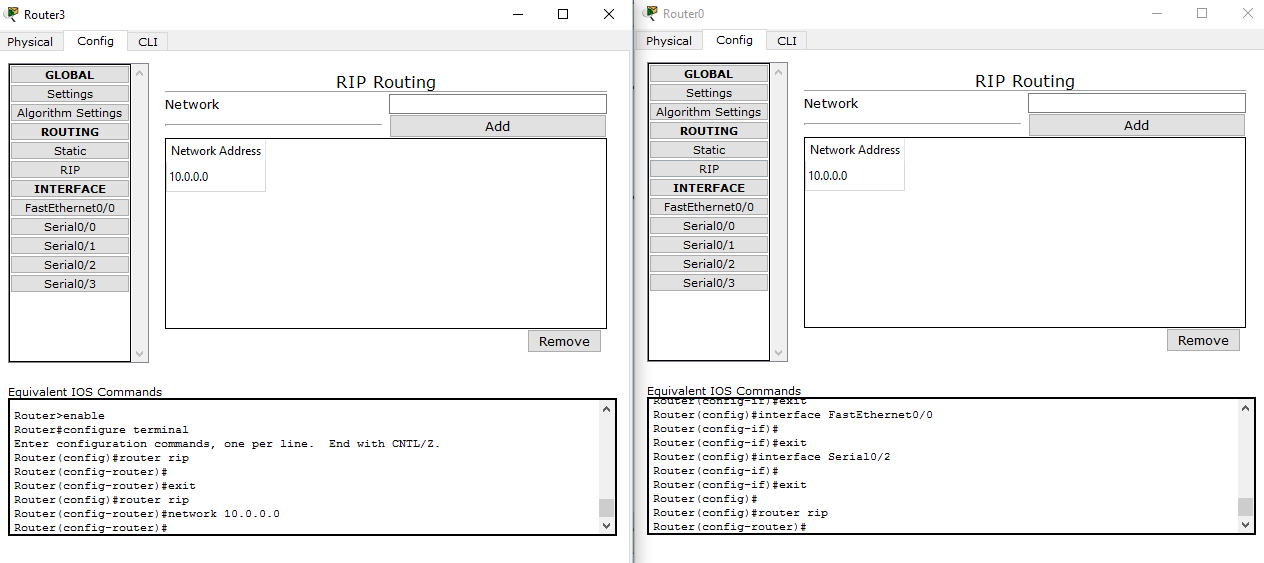
\includegraphics[width=\textwidth]{Ruteo_dinamico.PNG}
	\caption{Configuracion de ruteo dinamico en los router R0 y R3}
	\end{figure}\\
{\large \bf{Cuestionario: }}\\
	\begin{enumerate}
	    \item ¿Qué ventajas y desventajas se pueden apreciar en cada tipo de enrutamiento?\\\\
	    VENTAJAS:
	    Enrutamiento Estático:\\
	    \begin{itemize}
	    	\item El consumo de recursos del router es bajo.
	    	\item Es fácil de configurar en redes pequeñas.
	    \end{itemize}
	    Enrutamiento Dinámico:\\
	    \begin{itemize}
	    	\item En el mantenimiento de las rutas el encargado casi no debe participar.
	    	\item Esta configuración tiende a tener menos errores.
	    \end{itemize}
	    DESVENTAJAS:\\
	    Enrutamiento Estático:\\
	    \begin{itemize}
	    	\item Para redes grandes es complicado de configurar.
	    	\item La configuración es propensa a errores.
	    	\item La configuración, mantención y actualización de rutas se debe hacer manualmente.
	    	\item No permite una escalabilidad en caso de gran crecimiento de la topología.
	    Enrutamiento Dinámico:\\
	    \begin{itemize}
	    	\item El consumo de recursos del router es alto.
	    	\item Se requiere un conocimiento avanzado.
	    %(SIEMPRE SE PUEDEN AGREGAR MÁS)
	    \end{itemize}
            \item ¿En que se basa el enrutamiento dinámico para generar su ruta?\\\\
 
  	     
	\end{enumerate}
	
    
	
\chapter{Conclusión}
 
\begin{thebibliography}{x}
\bibitem{Website Osi} \textsc{Cisco },
\textit{cisco.utmetropolitana.edu.mx}
\textit{es.slideshare.net/eduardoelange/diferencias-entre-enrutamiento-esttico-y-dinmico}

\end{thebibliography}

\end{document}
